\chapter{Kapitel IV - NoSQL – Ausgewählte Systeme in Action}
\section{ArangoDB}
\subsection{Anwendungsszenarien}
Zur Betrachtung des praktischen Einsatzes von ArangoDB, haben wir drei verschiedene Anwendungsszenarien durchgeführt. Die Anwendungsszenarien sind so konzipiert, dass jedes Szenario einen Modelltyp des Multimodells von ArangoDB darstellt. Des Weiteren untersuchen wir zwei verschiedene Zugriffsfunktionen - Java und FOXX. Als Ergebnis untersuchen wir die Zugriffszeit der jeweiligen Zugriffsfunktionen auf die Datenbank.
\subsubsection{Anwendungsszenario 1 - Dokumentenbasiertes Szenario}
Um das dokumentenbasierte Datenmodell zu testen, wurde als Anwendungsszenario die Suche nach einen gewissen Wertes in Dokumenten erstellt. Bei dem vorgestellten Schema wird in diesen Szenario die Farbe von gewissen Autos gesucht. Beispiel: Alle Autos der Farbe Rot.
\subsubsection{Anwendungsszenarien 2 - Key-Value Szenario}
In diesen Szenario geht es darum die Vorteile des Key-Value-Modells, daher wird mit dem Nummernschild ein gewisses Auto so schenll wie möglich gesucht.
\subsubsection{Anwendungsszenarien 3 - Graph Szenario}
Das dritte Szenario testet das Graph Modell von ArangoDB. Hierfür wollen wir in diesen Szenario erfahren, wie viele Unfälle ein Automodell (Bspw. VOLVO) an den anderen Automodellen angerichtet hat. Am Ende wollen wir eine Übersicht von Modellen und die Anzahl der Unfälle erhalten.
\subsection{Umsetzung in Java}
\subsubsection{Datenbankzugriff}
\subsubsection{Schnittstelle nach Außen}
\subsubsection{Anwendungsszenario 1}
\subsubsection{Anwendungsszenario 2}
\subsubsection{Anwendungsszenario 3}
\subsection{Umsetzung in FOXX}
\subsubsection{Datenbankzugriff}
FOXX ist ein Framework, welches von ArangoDB angebot wird. Es dient dazu Microservices direkt in der Datenbank zu implementieren. Daher sind die Datenzugriffe sehr Nahe an der Datenbank und besonders performant. Um Beispielsweise auf die Auto-Datenbankcollection zuzugreifen, schreibt man bei FOXX folgenden Code:
\lstinputlisting[linerange={5-5}]{./src/index.js}
Diese Collection wird in den folgenden Szenarien gebraucht, um Abfragen zu tätigen.
\subsubsection{Schnittstelle nach Außen}
Als Microservice bietet FOXX eine HTTP-Schnittstelle, um den Zugriff von anderen Systemen zu ermöglichen. Diese Schnittstelle wurde von dem ArangoDB-Team bereitgestellt und wird in JavaScript implementiert. Es können zwar NodeJS Pakete benutzt werden, aber es werden nicht alle unterstützt, da zum Beispiel der Zugriff aufs Dateisystem verweigert wird.
\subsubsection{Anwendungsszenario 1}
\lstinputlisting[linerange={15-30}]{./src/index.js}
\subsubsection{Anwendungsszenario 2}
\lstinputlisting[linerange={32-60}]{./src/index.js}
\subsubsection{Anwendungsszenario 3}
\lstinputlisting[linerange={62-87}]{./src/index.js}
\subsection{Anwendung und Test}
Um die Implementierungen der Schnittstellen zur ArangoDB zu testen, werden die beiden Webservices (Java und FOXX) abgefragt. Das Frontend kann unter folgenden Link im Cluster erreicht werden: \texttt{http://10.20.110.61/team38/sdb-foxx-service/} \newline
Um zufällige Schwankungen abzufangen, werden bei jeden Szenario mehrere Requests gemacht und ein Durchschnittswert ermittelt. Die Tests der Anwendungsszenarien werden mit jeweils 100 Anfragen getestet. Daraus ergeben sich dann folgende Ergebnisse:
\begin{figure}[htbp] 
  	\centering
     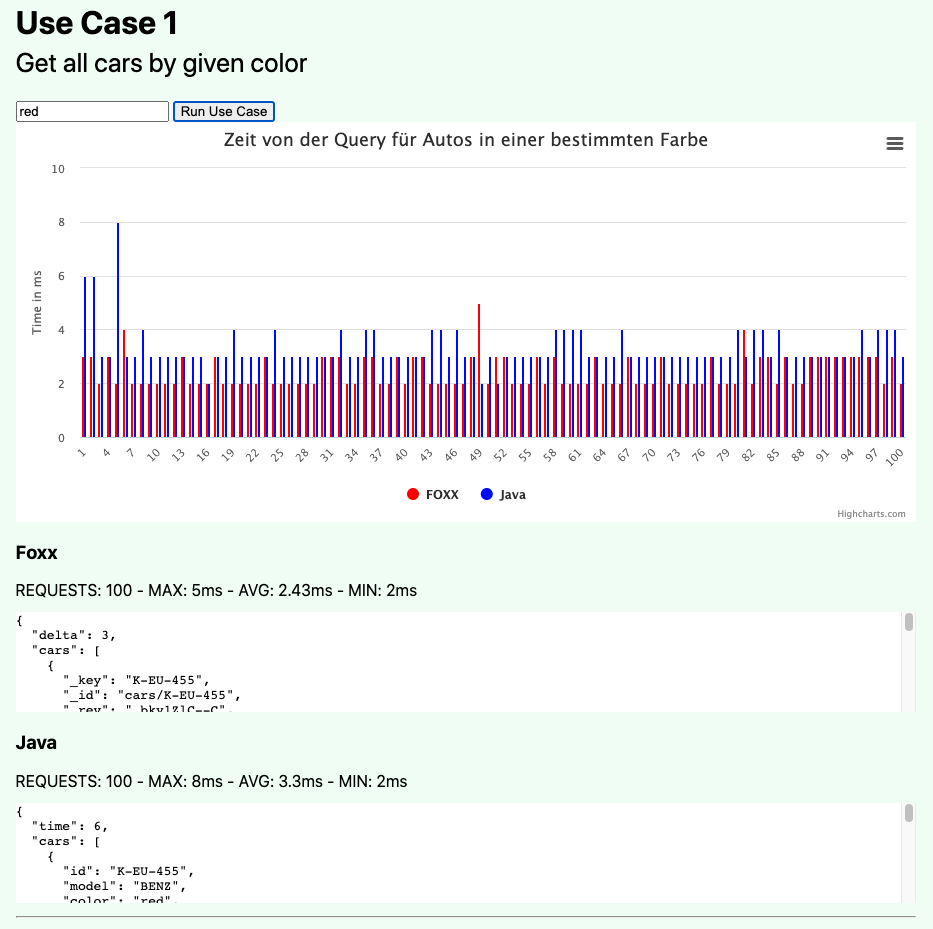
\includegraphics[width=1\textwidth]{./images/UseCase1.png}
 	\caption{Anwendungsszenario 1 Ergebnisse}
  \label{fig:DataSchema}
\end{figure}
\begin{figure}[htbp] 
  	\centering
     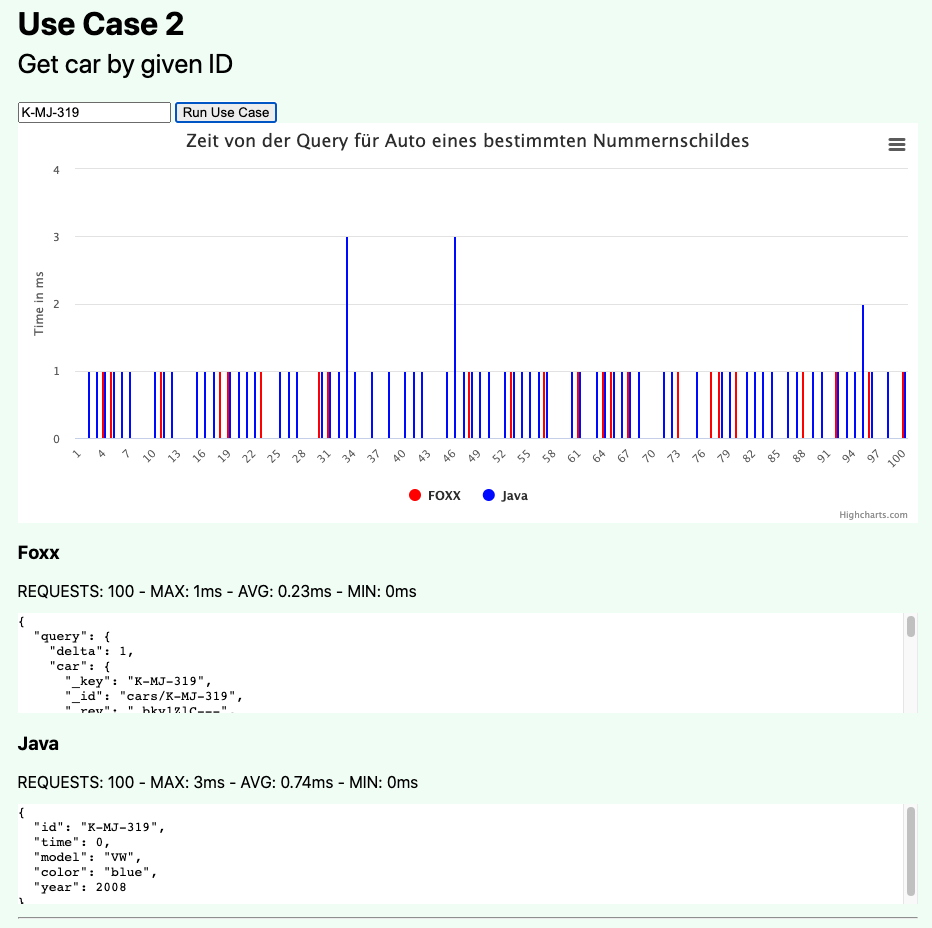
\includegraphics[width=1\textwidth]{./images/UseCase2.png}
 	\caption{Anwendungsszenario 2 Ergebnisse}
  \label{fig:DataSchema}
\end{figure}
\begin{figure}[htbp] 
  	\centering
     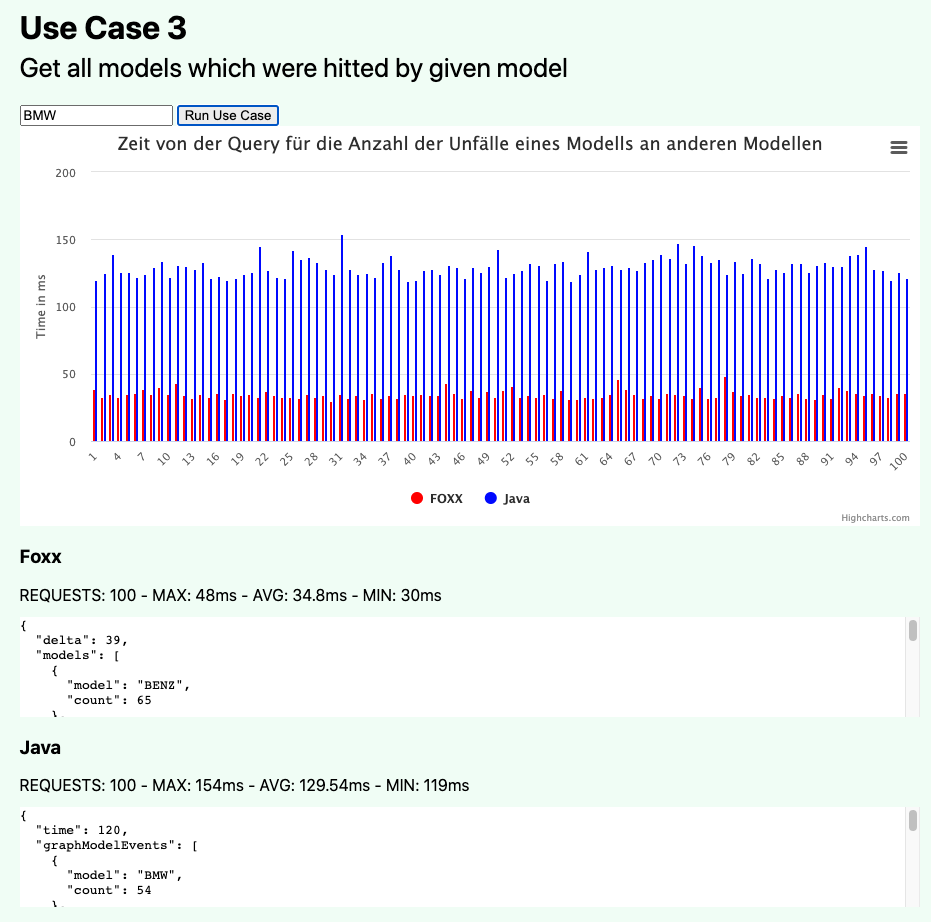
\includegraphics[width=1\textwidth]{./images/UseCase3.png}
 	\caption{Anwendungsszenario 3 Ergebnisse}
  \label{fig:DataSchema}
\end{figure}
\subsection{Fazit}
Bei allen Szenarien lässt sich erkennen, dass FOXX einen schelleren Zugriff auf die Datenbank hat als Java. Erklären lässt sich dies bei Szenario 1 und 2 durch die Latenz der Übertragung zwischen Master-Node (dort läuft Java) und Node 4 (ArangoDB-Datenbank-Koordinator). \newline
Bei Anwendungsszenario 3 fällt auf, dass der Unterschied zwischen FOXX und Java sehr groß ist. Jedoch lässt sich der Unterschied nicht mit der Latenz des Zugriffs erklären. Man kann also davon ausgehen, dass FOXX schneller komplexe Abfragen umsetzen kann. \newline
Daraus lässt schließen, dass nicht nur die Latenz zwischen den Servern bei Szenario 1 und 2 den Unterschied gemachten haben, sondern auch die Zugriffsschnittstelle der beiden Anwendungen. Man kann also sagen, dass die datenbanknahe Implementierung der FOXX-Microservices einen großen Vorteil bei der Abfragegeschwindigkeit bringen.